\documentclass{sigchi}

% Use this command to override the default ACM copyright statement (e.g. for preprints). 
% Consult the conference website for the camera-ready copyright statement.
\toappear{
  Submitted for review.
}

% Arabic page numbers for submission. 
% Remove this line to eliminate page numbers for the camera ready copy
\pagenumbering{arabic}


% Load basic packages
\usepackage{balance}  % to better equalize the last page
\usepackage{graphicx} % for EPS, load graphicx instead
\usepackage{times}    % comment if you want LaTeX's default font
\usepackage{url}      % llt: nicely formatted URLs
\usepackage{subfigure}


%\linespread{2}

% llt: Define a global style for URLs, rather that the default one
\makeatletter
\def\url@leostyle{%
  \@ifundefined{selectfont}{\def\UrlFont{\sf}}{\def\UrlFont{\small\bf\ttfamily}}}
\makeatother
\urlstyle{leo}


% To make various LaTeX processors do the right thing with page size.
\def\pprw{8.5in}
\def\pprh{11in}
\special{papersize=\pprw,\pprh}
\setlength{\paperwidth}{\pprw}
\setlength{\paperheight}{\pprh}
\setlength{\pdfpagewidth}{\pprw}
\setlength{\pdfpageheight}{\pprh}

% Make sure hyperref comes last of your loaded packages, 
% to give it a fighting chance of not being over-written, 
% since its job is to redefine many LaTeX commands.
\usepackage[pdftex]{hyperref}
\hypersetup{
pdftitle={SIGCHI Conference Proceedings Format},
pdfauthor={LaTeX},
pdfkeywords={SIGCHI, proceedings, archival format},
bookmarksnumbered,
pdfstartview={FitH},
colorlinks,
citecolor=black,
filecolor=black,
linkcolor=black,
urlcolor=black,
breaklinks=true,
}

% create a shortcut to typeset table headings
\newcommand\tabhead[1]{\small\textbf{#1}}


% End of preamble. Here it comes the document.
\begin{document}

\title{SIGCHI Conference Proceedings Format}

\numberofauthors{2}
\author{
  \alignauthor 1st Author Name\\
    \affaddr{Affiliation}\\
    \affaddr{Address}\\
    \email{e-mail address}\\
  \alignauthor 2nd Author Name\\
    \affaddr{Affiliation}\\
    \affaddr{Address}\\
    \email{e-mail address}\\
}

\maketitle

\begin{abstract}
\end{abstract}

\keywords{
  Guides; instructions; author's kit; conference publications;
  keywords should be separated by a semi-colon.
}

\category{H.5.m.}{Information Interfaces and Presentation (e.g. HCI)}{Miscellaneous}

\section{Introduction}

% Abstract Hidden Markov Model for online continuous gesture recognition with
% unbounded and unsegmented RGB and depth video sequences. 

\section{Related Work}
Bag-of-feature approach is similar to the bag-of-word approach in document classification.
To represent an image using BoW model, an image can be treated as a document. Similarly,
``words'' in images need to be identified too. To achieve this, it usually includes
following three steps: feature detection, feature description and code book generation~\cite{fei2005}.
In the bag-of-word approach for document classification, the notion of order of words is lost
~\cite{Russell2003}. Higher-order $n$-gram models maintain some local notion of word order.

Heng et al. did an evaluation of several feature detectors and descriptors for action
recognition in video sequences~\cite{wang2009}. They used the same bag-of-features SVM classification
method for all the feature detector and descriptor combinations.
Codebook With the bag of words

SVM does not usually handle time series data. To use SVM for time series, one
can concatenate the input in a time series into one long vector sample. scale
short time
action recognition

Any HHMM can be converted to regular HMM by creating an HMM state for every leaf in the HHMM
state transition diagram~\cite{murphy02}. Both HHMM and HMM have advantages and disadvantages. Advantages for HHMM
over a mixture of HMMs model.
\begin{itemize}
  \item Can share substructures ($S_t$) across different HMMs, but not in the mixture of HMMs model.
  \item HHMM can provide a mult-A flat HMM cannot easily provide
\end{itemize}

Advantages of HMM
\begin{itemize}
  \item Can specify more constraints in the the parameters, i.e. use Bakis model. to reduce the total number of parameters
It is harder to impose Bakis model to HHMM since the hidden states are shared. The state transition probability for $S_t$ in HHMM
is $|S|^2 \times |G| $. In mixture HMMs model, it is $k\times |S|\times|G|$ where $k$ is the number of states a state can transit to.
\end{itemize}

If we do not constrain the transition in the hidden states $S_t$, HHMM may have a fewer number of parameters because of the states sharing.
If we constrain the transition, specifying more structures in the sub HMMs, the mixture of HMMs can have fewer number of parameters.

Training HMMs separately and combining them into HHMM for gesture inference. No across-gesture sharing (of hidden states)

dynamic time warping

\subsection{Hand Tracking}
Marcos-Ramiro et al. ~\cite{marcos2013} develop a method of computing hand likelihood maps based on RGB videos. Optical flow
hands show more movement. Our method is very similar to their approach but we combine both RGB images and depth images to compute
the gesture salience map. They hypothesized that given a frontal, static camera pointing to the upper body of a person, hands are
normally the parts of the image that show more movement. The two strong indicators are:

Space-time interest point
\section{Implementation Details}
PCA reduction. The features are in the PC space, so they should have small correlations.
So we set the covariance matrices for the Gaussian CPD to be diagonal.


Local space-time features capture characteristic shape and motion in video and
provide relatively independent representation of events with respect to their
spatio-temporal shifts and scales. \cite{wang-spatio-2009}


\cite{wang-spatio-2009}

Kinect skeleton tracking methods random forest

\section{System Overview}
Our online continuous hand gesture recognition framework consists mainly two parts: feature
extraction and gesture classification.

Feature extraction on video sequences can be broken down into two steps: 1)
detect points of interest by maximizing certain salience functions; 2) compute
feature descriptors to capture shape and motion in the neighborhoods of selected
points using image measurements~\cite{wang-spatio-2009}.

For hand gesture recognition, the points of interest are certainly the hands. While the skeleton tracking provided
by the Kinect SDK is quite robust most of the time, its error for the hand joint tracking increases when
the hands are close to the body or move quickly (see Figure~\ref{fig:compare-skeleton}). As a result, we
develop the gesture salience detection method to locate the gesturing hand more accurately.
 
\section{Gesture Salience Detection}

Similar to Marcos-Ramiro et al.~\cite{marcos2013}, we define gesture salience as a function of 
the closeness of the motion to the observer (e.g., the camera) and the magnitude of the motion.

For a given data frame from the RGB-D camera, we combine both the RGB and the depth data to 
compute gesture salience. Both the RGB and the depth data can be noisy. RGB cameras are sensitive to lighting conditions (cite).
Skin color based detection can be sensitive to the clothes users wear. Depth cameras based on 
structured light sensors, such as the first generation Kinect sensor, compare the projected infra-red pattern
with the reflected one to determine depth~\cite{welsh:2011}. As a result, they do not work well on 
objects that are highly reflective (mirrors and shiny metal) or highly absorptive (fluffy and/or dark materials such as human hair)
\footnote{\url{http://msdn.microsoft.com/en-us/library/hh855356.aspx}}. By combining the two,
the overall gesture salience detection can be more robust to noise.

The following are the detailed steps of our gesture salience detection method for each frame. 
We show the illustrations in Figure~\ref{fig:gesture-salience}. 

\subsection{Skin Segmentation}
We use an off-the-shelf simple skin color detection method which is not trained on our data set to do a binary segmentation. The reason is
to make the method generalizable to any users and environment. We compute a binary skin mask, $M^S$, based on the RGB image converted into YCrCb
color space.  We also find the user mask, $M^U$ obtained from the Kinect SDK based on the depth image. 
We then align $M^S$ with $M^U$ and find their intersection $M^{S\wedge U}$, which indicates the skin region on the user (Figure~\ref{fig:skin-mask}).

\subsection{Motion Detection}
Similar to Cutler and Turk~\cite{cutler1998}, we compute the motion mask for the current depth frame based on 3 frames. We first filter each 
depth frame by the user and skin mask $M^{S\wedge U}$ at time $t$ to obtain $D_t$. 
Equation~(\ref{eq:motion-mask}) computes the binary mask, $M_{t\vee t-1}^M$, indicating moved pixels at either time $t$ or $t - 1$ (Figure~\ref{fig:motion-mask}).
$D_{t\vee t-1}^{D}$ is the absolute difference between $D_t$ and $D_{t-1}$, and $T$ is the threshold operator that filters out small change in depth value 
(we set the threshold to be 15mm). 
To obtain the motion mask, $M_{t}^M$ for time $t$ only, we use $M_{t-1\vee t-2}^M$, the motion mask for $t-1$ and $t-2$ as well (see Equation~(\ref{eq:motion-mask-t-1})-(\ref{eq:motion-mask-t}),
symbols $\wedge$ and $\oplus$ are the AND and XOR operators respectively).
\begin{align}
M_{t\vee t-1}^M &= T(D_{t\vee t-1}^{D}) \label{eq:motion-mask} \\
M_{t-1}^M &= M_{t\vee t-1}^M \wedge M_{t-1\vee t-2}^M \label{eq:motion-mask-t-1}\\
M_{t}^M &= M_{t\vee t-1}^M \oplus M_{t-1}^M \label{eq:motion-mask-t}
\end{align}

\subsection{Salience Map}
We apply histogram equalization to both $D_t$ and $D_{t\vee t-1}^{D}$ to obtain cumulative distributions $H_t$ and $H_{t\vee t-1}^D$.
$H_t$ represents the probability of salience given a depth value and $H_{t\vee t-1}^D$ represents the probability of salience given
a depth difference value. The lower the depth value or the higher the depth difference value, the higher the salience probability.
Finally the salience map (Figure~\ref{fig:salience}) can by computed for each pixel $(x, y)$ as
\begin{align}
S(x, y) = H_t(D_t(x, y)) \times H_{t\vee t-1}^D(D_t^D(x, y)) \times M_t^M
\end{align}
The multiplication of the binary motion mask $M_t^M$ allows us to only consider the motion due to the user at $t$.
 
\subsection{Salience Detection}
The final step of locating the most salient region in a frame is finding the contour, $C$, from the salience map $S$ that has a perimeter greater than the smallest possible
hand perimeter and with the highest average salience for all the pixels in side the contour.

When motion is slow, the motion mask usually indicates the edge of the moving object. As a result, the center of $C$
may not be the center of the moving object (in our case, the user's hand). Hence, we use 2 iterations of Camshift~\cite{Bradski98} on the 
depth image $D_t$ with a start search location at then center of $C$ to refine the final location of gesture salience (Figure~\ref{fig:camshift}).

\begin{figure*}[tb]
\centering
\hspace{-0.6em}%
\subfigure[]{
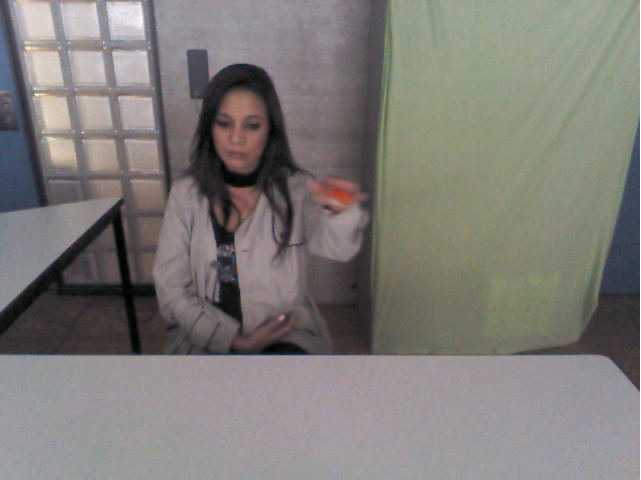
\includegraphics[width=0.195\linewidth]{figure/color.PNG}\hspace{-0.6em}%
\label{fig:color}
}
\subfigure[]{
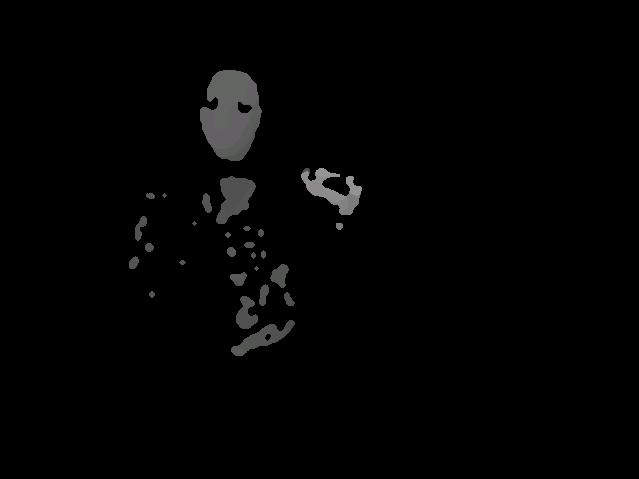
\includegraphics[width=0.195\linewidth]{figure/depth.PNG}\hspace{-0.6em}
\label{fig:skin-mask}
}
\subfigure[]{
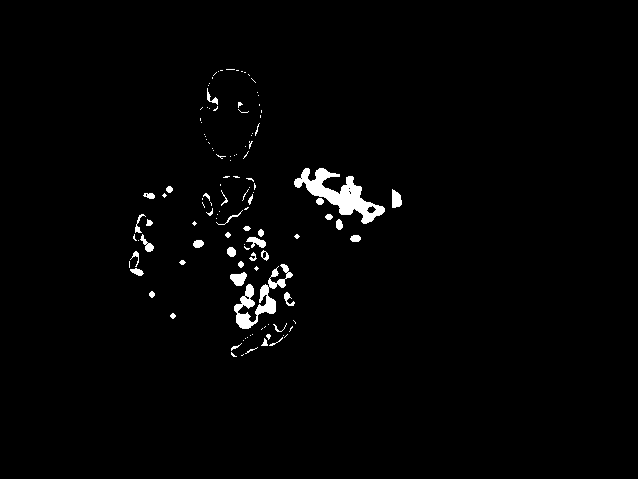
\includegraphics[width=0.195\linewidth]{figure/motion-mask1.PNG}\hspace{-0.6em}
\label{fig:motion-mask}
}
\subfigure[]{
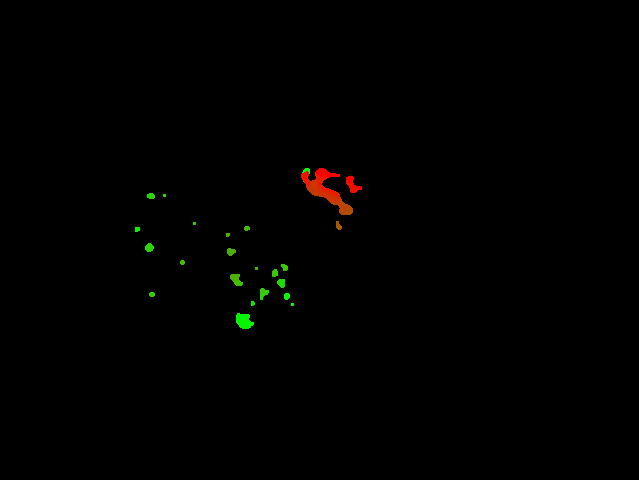
\includegraphics[width=0.195\linewidth]{figure/salient-map.PNG}\hspace{-0.6em}
\label{fig:salience}
}
\subfigure[]{
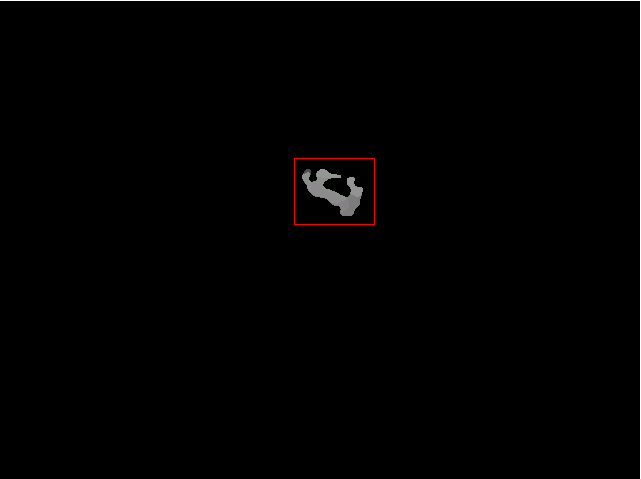
\includegraphics[width=0.198\linewidth]{figure/bounding-box.PNG}
\label{fig:camshift}
}
\caption{Gesture salience detection steps: \subref{fig:color} RGB image under low lighting condition;
\subref{fig:skin-mask} depth map $D_t$ filtered by skin and user mask, $M^{S\wedge U}$. False detection of skin due to
clothes color similar to skin color; \subref{fig:motion-mask} motion mask,  $M_{t\vee t-1}^M$, indicating moved pixels for time $t$ and $t-1$;
\subref{fig:salience} salience map with red color indicating high probability of the salience; \subref{fig:camshift} final gesture salience location.}
\label{fig:gesture-salience}
\end{figure*}

Figure~\ref{fig:compare-skeleton} compares the results of gesture salience detection for hand gestures with the skeleton tracking results
from the Kinect SDK.
\begin{figure*}
\centering
\subfigure[]{
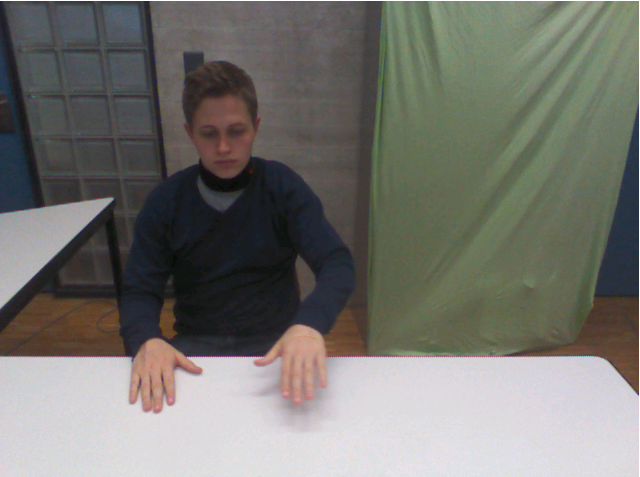
\includegraphics[width=0.24\linewidth]{figure/rotate-color.PNG} \hspace{-0.6em}
}
\subfigure[]{
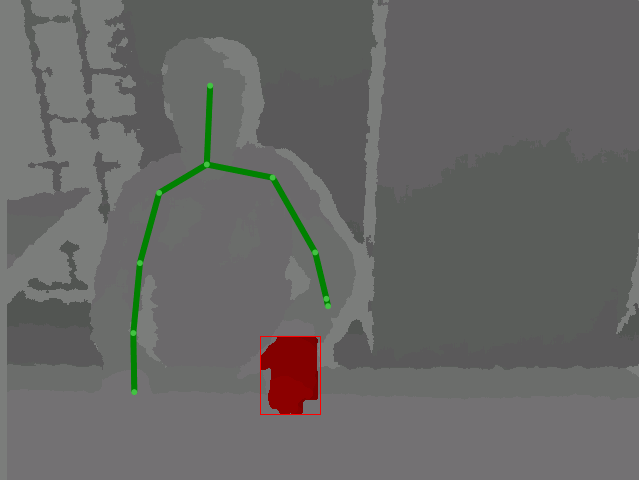
\includegraphics[width=0.24\linewidth]{figure/rotate-depth.PNG} \hspace{-0.6em}
}
\subfigure[]{
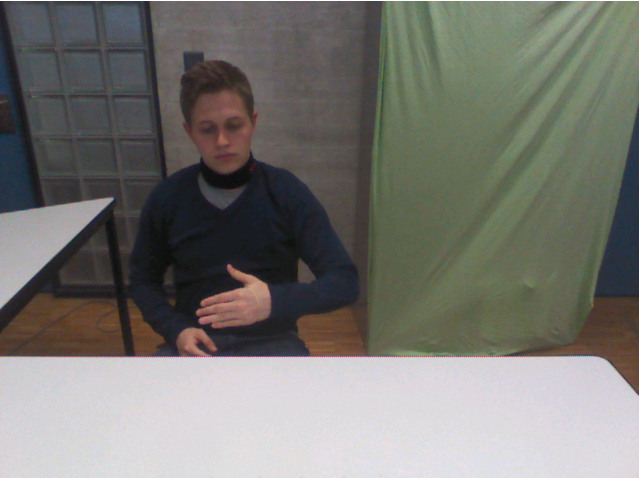
\includegraphics[width=0.24\linewidth]{figure/near-body-color.PNG} \hspace{-0.6em}
}
\subfigure[]{
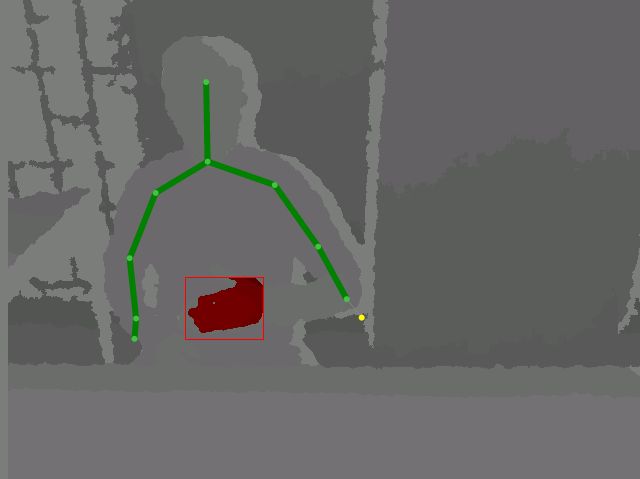
\includegraphics[width=0.24\linewidth]{figure/near-body-depth.PNG} \hspace{-0.6em}
}
\caption{Comparison between gesture salience detection for hand gestures and skeleton tracking from the Kinect SDK. The green lines are
the skeleton tracking results. The red region is the detected salient gesture region using our method.}
\label{fig:compare-skeleton}
\end{figure*}
% \subsection{HMM Training}
% 
% Compute termination probability $P(END|S_T)$
% 
% 
% \subsection{Online Inference}

\section{Online Continuous Gesture Recognition}
\section{Experimental Evaluation}

% \subsection{Data Set}
% data set has both lighting conditions: normal and low intensity. IMU sensors, not used. Intrusive.
% 13 gesture phases and a random guess accuracy would be 7.8\%.
% 
% 8 users
\subsection{Comparison of Feature Detection Methods}
% \begin{table}
%   \centering
%   \begin{tabular}{|c|c|c|}
%     \hline
%     \tabhead{Objects} &
%     \multicolumn{1}{|p{0.3\columnwidth}|}{\centering\tabhead{Caption --- pre-2002}} &
%     \multicolumn{1}{|p{0.4\columnwidth}|}{\centering\tabhead{Caption --- 2003 and afterwards}} \\
%     \hline
%     Tables & Above & Below \\
%     \hline
%     Figures & Below & Below \\
%     \hline
%   \end{tabular}
%   \caption{Table captions should be placed below the table.}
%   \label{tab:table1}
% \end{table}

% \textbf{Dense} sampling extracts
% per frame accuracy
% Skin and skeleton method finds the skin contour closest to the right hand joint from
% the skeleton tracking result provided by Microsoft's Kinect SDK.
%   
% We use the same feature descriptor HOG 4, 9, pca reduction
\begin{table}
\centering
\begin{tabular}{|l|l|l|}
\hline
\tabhead{Feature detector} & {\tabhead{Accuracy (std.)}} & {\tabhead{F1 (std.)}}\\
\hline
Dense sampling upper body & 68.0\% (4) & 57.7\% (8)\\
\hline
Skin \& skeleton & 72.1\% (16) & 64.7\% (11) \\
\hline
Salience & \textbf{76.7\%} (4) & \textbf{69.3\%} (6) \\
\hline
\end{tabular}
\caption{}
\end{table}

\begin{table}
\centering
\begin{tabular}{|l|l|l|}
\hline
\tabhead{Hand pose feature} & {\tabhead{Accuracy (std.)}} & {\tabhead{F1 (std.)}}\\
\hline
No hand pose feature & 76.5\% (5) & 68.4\% (7)\\
\hline
Use hand pose feature  & \textbf{76.7\%} (4) & \textbf{69.3\%} (6) \\
\hline
\end{tabular}
\caption{}
\end{table}

\subsection{Comparison of Recognition Training Methods}
% Graph search?
% Same salience feature detector and descriptor.
% HMM with reset, does not learn the transition probability between states across gestures.
% Can reduce the number of parameters to learn.
% reset S state

\begin{table}[t]
\centering
\begin{tabular}{|l|l|l|}
\hline
\tabhead{Training method} & {\tabhead{Accuracy (std.)}} & {\tabhead{F1 (std).}}\\
\hline
HMM & 50.6\% (17) & 55.6\% (8) \\
\hline
AHMM & \textbf{76.7\%} (4) & \textbf{69.3\%} (6) \\
\hline
\end{tabular}
\caption{}
\end{table}

\begin{table}[t]
\centering
\begin{tabular}{|l|l|l|}
\hline
\tabhead{Inference} & {\tabhead{Accuracy (std.)}} & {\tabhead{F1 (std).}}\\
\hline
Offline & 76.7\% (4) & 69.3\% (6) \\
\hline
Online (lag = 16 frames) & \textbf{76.9\%} (3) & \textbf{65.2\%} (9) \\ 
\hline
\end{tabular}
\caption{}
\end{table}


\section{Future Work}
% Do away from skin color, what if the user wear glove, or like in the data set,
% holding something in the hand.

\section{Conclusion}

% It is important that you write for the SIGCHI audience.  Please read
% previous years' Proceedings to understand the writing style and
% conventions that successful authors have used.  It is particularly
% important that you state clearly what you have done, not merely what
% you plan to do, and explain how your work is different from previously
% published work, i.e., what is the unique contribution that your work
% makes to the field?  Please consider what the reader will learn from
% your submission, and how they will find your work useful.  If you
% write with these questions in mind, your work is more likely to be
% successful, both in being accepted into the Conference, and in
% influencing the work of our field.

% Balancing columns in a ref list is a bit of a pain because you
% either use a hack like flushend or balance, or manually insert
% a column break.  http://www.tex.ac.uk/cgi-bin/texfaq2html?label=balance
% multicols doesn't work because we're already in two-column mode,
% and flushend isn't awesome, so I choose balance.  See this
% for more info: http://cs.brown.edu/system/software/latex/doc/balance.pdf
%
% Note that in a perfect world balance wants to be in the first
% column of the last page.
%
% If balance doesn't work for you, you can remove that and
% hard-code a column break into the bbl file right before you
% submit:
%
% http://stackoverflow.com/questions/2149854/how-to-manually-equalize-columns-
% in-an-ieee-paper-if-using-bibtex
%
% Or, just remove \balance and give up on balancing the last page.
%
\balance

% If you want to use smaller typesetting for the reference list,
% uncomment the following line:
% \small
\bibliographystyle{acm-sigchi}
\bibliography{gesture}
\end{document}
